\begin{frame}{Verification of ChatGPT Responses (RQ3)}
    Participants were presented with conversations with ChatGPT where it was asked
    \begin{itemize}
        \item Suggestions 
        \item More detail about a specific situation
        \item Reliability in SE real-world situations
    \end{itemize}
\end{frame}

\begin{frame}{Key Findings}
    \begin{center}
        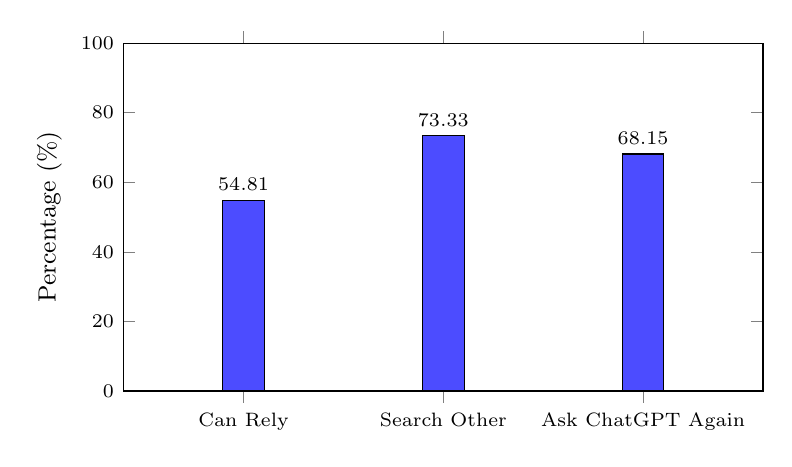
\begin{tikzpicture}
            \begin{axis}[
                ybar,
                bar width=15pt,
                width=0.8\textwidth,
                height=6cm,
                symbolic x coords={Can Rely, Search Other, Ask ChatGPT Again},
                xtick=data,
                xlabel={},
                ylabel={Percentage (\%)},
                ymin=0, ymax=100,
                nodes near coords,
                nodes near coords align={vertical},
                every node near coord/.append style={font=\scriptsize},
                enlarge x limits=0.3,
                ylabel style={font=\small},
                xlabel style={font=\small},
                ticklabel style={font=\scriptsize}
            ]
                % Data points
                \addplot[fill=blue!70] coordinates {
                    (Can Rely, 54.81)
                    (Search Other, 73.33)
                    (Ask ChatGPT Again, 68.15)
                };
            \end{axis}
        \end{tikzpicture}
    \end{center}
\end{frame}


%------------------------------------------------

\section{CID: ChatGPT Incorrectness Detector}

%------------------------------------------------

\begin{frame}
    \frametitle{Introducing CID}
    \begin{itemize}
        \item CID (ChatGPT Incorrectness Detector) tool
uses iterative prompting to capture ChatGPT’s inconsistency in a
similar fashion to an actual Crime Investigation Department (CID).
    \end{itemize}
\end{frame}

\begin{frame}{CID Tool Components}
    \begin{center}
    \begin{tikzpicture}
        % Main CID node
        \node[draw, circle, minimum size=1cm, thick, color=blue!70,visible on=<1->] (CID) at (7, 6.5) {CID};

        % Enquirer node
        \node[draw, rectangle, rounded corners=3pt, thick, color=red!80, below left=1.5cm and 2.5cm of CID,visible on=<2->] (Enquirer) {Enquirer};

        % Challenger node
        \node[draw, rectangle, rounded corners=3pt, thick, color=purple!80, below=2.5cm of CID,visible on=<3->] (Challenger) {Challenger};

        % Decider node
        \node[draw, rectangle, rounded corners=3pt, thick, color=orange!80, below right=1.5cm and 2.5cm of CID,visible on=<4->] (Decider) {Decider};

        % Connecting arrows
        \draw[->, thick, color=blue!70,visible on=<2->] (CID) -- (Enquirer);
        \draw[->, thick, color=blue!70,visible on=<3->] (CID) -- (Challenger);
        \draw[->, thick, color=blue!70,visible on=<4->] (CID) -- (Decider);
    \end{tikzpicture}
    \end{center}
\end{frame}

% \begin{frame}{dummy}
% \begin{tikzpicture}
%     \matrix (magic) [matrix of nodes,ampersand replacement=\&, column sep=7mm, row sep=5mm]{
%         \node (se) [draw,shape=rectangle,visible on=<5->] {Existence Forte}; \&
%         \node (yw) [draw,shape=circle,visible on=<1->] {Yamada-watanab}; \&
%         \node (ul) [draw,shape=rectangle,visible on=<9->] {Unicité en Loi}; \\
%         \node (d1) [draw,shape=circle,visible on=<6->] {Définition}; \& 
%         \&   
%         \node (d2) [draw, shape=circle,visible on=<8->] {Définition}; \\
%         \node (we) [draw, shape=rectangle,visible on=<2->] {Existence Faible}; \&
%         \node (ec) [draw, shape=circle,visible on=<10->] {Engelbert-Cherny}; \& 
%         \node (pu) [draw, shape=rectangle,visible on=<3->] {Unicité Trajectorielle}; \\
%     };
%     \draw[->, thick,visible on=<6->] (se) -- (d1); \draw[->, thick,visible on=<7->]  -- (we);
%     \draw[->, thick,visible on=<4->] (we) -- (yw); \draw[->, thick,visible on=<5->] (yw) -- (se);
%     \draw[->, thick,visible on=<11->] (se) -- (ec); \draw[->, thick,visible on=<11->] (ul) -- (ec);
%     \draw[->, thick,visible on=<12->] (ec) -- (pu); \draw[->, thick,visible on=<4->] (pu) -- (yw);
%     \draw[->, thick,visible on=<8->] (pu) -- (d2); \draw[->, thick,visible on=<9->] (d2) -- (ul);
% \end{tikzpicture}
    
% \end{frame}

\begin{frame}{}
    \begin{tikzpicture}
        \draw [ color={rgb,255:red,40; green,84; blue,154} , line width=1pt, visible on=<1->] (4,11.5) rectangle (6.5,10.25) node[pos=.5] {Enquirer};
        \draw [color={rgb,255:red,45; green,169; blue,155} , line width=0.7pt, rounded corners = 11.3, visible on=<3->] (8,10.5) rectangle (10.5,11.25) node[pos=.5] {\tiny{Explanations}};;
        % \draw [ color={rgb,255:red,40; green,84; blue,154} , line width=1pt ] (4.25,8) rectangle (6.25,6.5)  node[pos=.5] {\footnotesize{Challenger}};;;
        % \draw [ color={rgb,255:red,45; green,169; blue,155} , line width=0.7pt, rounded corners = 11.3] (8.25,7.5) rectangle (10.5,6.75) node[pos=.5] {\tiny{Challenge responses}};;;
        % \draw [ color={rgb,255:red,40; green,84; blue,154} , line width=1pt ] (12.5,10.25) rectangle (14.5,8.5) node[pos=.5] {Decider};;
        \draw [ color={rgb,255:red,45; green,169; blue,155} , line width=0.7pt, rounded corners = 11.3,visible on=<2->] (4,13) rectangle (6.5,12.25) node[pos=.5] {\tiny{ChatGPT response}};
        % \draw [ color={rgb,255:red,45; green,169; blue,155} , line width=0.7pt, rounded corners = 11.3] (11.75,12.5) rectangle (15,11.75) node[pos=.5] {\tiny{Explanation-wise correctness}};
        \draw [->, thick, visible on=<2->] (5.25,12.25) -- (5.25,11.5);
        \draw [->, thick, visible on=<3->] (6.5,11) -- (8,11);
        % \draw [short, thick] (9.25,10.5) -- (9.25,9.25);
        % \draw [short, thick] (9.25,9.25) -- (5.5,9.25);
        % \draw [->, thick] (5.5,9.25) -- (5.5,8);
        % \draw [->, thick] (6.25,7.25) -- (8.25,7.25);
        % \draw [->, thick] (10.5,7.25) -- (12.5,9.25);
        % \draw [->, thick] (10.5,10.75) -- (12.5,9.25);
        % \draw [->, thick] (13.5,10.25) -- (13.5,11.75);
    \end{tikzpicture}
\end{frame}

%------------------------------------------------

% \begin{frame}
%     \frametitle{CID Components}
%     \begin{figure}
%         \centering
%         \begin{tikzpicture}[node distance=1.5cm]
%             % Nodes
%             \node (start) [startstop] {Start};
%             \node (enquirer) [process, below of=start] {ENQUIRER};
%             \node (challenger) [process, below of=enquirer] {CHALLENGER};
%             \node (decider) [process, below of=challenger] {DECIDER};
%             \node (end) [startstop, below of=decider] {End};
%             % Arrows
%             \draw [arrow] (start) -- (enquirer);
%             \draw [arrow] (enquirer) -- (challenger);
%             \draw [arrow] (challenger) -- (decider);
%             \draw [arrow] (decider) -- (end);
%         \end{tikzpicture}
%         \caption{Overview of CID Tool Workflow}
%     \end{figure}
% \end{frame}

%------------------------------------------------

\begin{frame}
    \frametitle{ENQUIRER Component}
    \begin{itemize}
        \item \footnotesize{The ENQUIRER targets to obtain ChatGPT’s initial reasoning behind the
base-response that can be useful to reveal any inconsistency in
the next steps of interrogation.} \pause
        \item \footnotesize{Asks ChatGPT to provide separate reasoning for each piece of information by using the following prompt.} \pause
        \begin{center}
        \begin{minipage}{0.8\textwidth}
            \begin{block}{\footnotesize{Enquiring ChatGPT}}
                \footnotesize{Justify your answer. If the answer has multiple
pieces of information, provide separate reasoning for each of them.}
            \end{block}
        \end{minipage}
        \end{center}
    \end{itemize}
\end{frame}

% %------------------------------------------------

\begin{frame}{}
    \begin{tikzpicture}
        \draw [ color={rgb,255:red,40; green,84; blue,154} , line width=1pt, visible on=<1->] (4,11.5) rectangle (6.5,10.25) node[pos=.5] {Enquirer};
        \draw [color={rgb,255:red,45; green,169; blue,155} , line width=0.7pt, rounded corners = 11.3, visible on=<1->] (8,10.5) rectangle (10.5,11.25) node[pos=.5] {\tiny{Explanations}};;
        \draw [ color={rgb,255:red,40; green,84; blue,154} , line width=1pt , visible on=<1->] (4.25,8) rectangle (6.25,6.5)  node[pos=.5] {\footnotesize{Challenger}};;;
        \draw [ color={rgb,255:red,45; green,169; blue,155} , line width=0.7pt, rounded corners = 11.3, visible on=<3->] (8.25,7.5) rectangle (10.5,6.75) node[pos=.5] {\tiny{Challenge responses}};;;
        % \draw [ color={rgb,255:red,40; green,84; blue,154} , line width=1pt ] (12.5,10.25) rectangle (14.5,8.5) node[pos=.5] {Decider};;
        \draw [ color={rgb,255:red,45; green,169; blue,155} , line width=0.7pt, rounded corners = 11.3,visible on=<1->] (4,13) rectangle (6.5,12.25) node[pos=.5] {\tiny{ChatGPT response}};
        % \draw [ color={rgb,255:red,45; green,169; blue,155} , line width=0.7pt, rounded corners = 11.3] (11.75,12.5) rectangle (15,11.75) node[pos=.5] {\tiny{Explanation-wise correctness}};
        \draw [->, thick, visible on=<1->] (5.25,12.25) -- (5.25,11.5);
        \draw [->, thick, visible on=<1->] (6.5,11) -- (8,11);
        \draw [short, thick, visible on=<2->] (9.25,10.5) -- (9.25,9.25);
        \draw [short, thick, visible on=<2->] (9.25,9.25) -- (5.5,9.25);
        \draw [->, thick, visible on=<2->] (5.5,9.25) -- (5.5,8);
        \draw [->, thick, visible on=<3->] (6.25,7.25) -- (8.25,7.25);
        % \draw [->, thick] (10.5,7.25) -- (12.5,9.25);
        % \draw [->, thick] (10.5,10.75) -- (12.5,9.25);
        % \draw [->, thick] (13.5,10.25) -- (13.5,11.75);
    \end{tikzpicture}
\end{frame}

\begin{frame}{Challenger Components}
    \begin{center} % Center the entire tikzpicture
        \begin{tikzpicture}[scale=0.8, every node/.style={transform shape}]
            % Main Challenger node
            \node[draw, circle, minimum size=0.8cm, thick, color=purple!80, visible on=<1->] (Challenger) at (0, 2) {Challenger};

            % Basic Challenger node (red)
            \node[draw, rectangle, rounded corners=3pt, thick, color=goldenrod!80, below left=1cm and 1.5cm of Challenger, visible on=<2->] (Basic) {Basic Challenger};

            % Mutation Challenger node (purple)
            \node[draw, rectangle, rounded corners=3pt, thick, color=goldenrod!80, below right=1cm and 1.5cm of Challenger, visible on=<3->] (Mutation) {Mutation Challenger};

            % Connecting arrows
            \draw[->, thick, color=purple!80, visible on=<2->] (Challenger) -- (Basic);
            \draw[->, thick, color=purple!80, visible on=<3->] (Challenger) -- (Mutation);
        \end{tikzpicture}
    \end{center}
\end{frame}

\begin{frame}
    \frametitle{Basic Challenger}
    \begin{itemize}
        \item \footnotesize{We first ask three basic challenge questions
to ChatGPT: \emph{Why?, How?, Really?} for each explanation $(E_i
)$ of its
base-response $(R_B)$.}
        \pause
        \item \footnotesize{The basic challenger leverages a separate LLM. } \pause
        \item \footnotesize{To replicate a separate LLM, we used ChatGPT with a new separate
session. The motive for using a separate session of ChatGPT is
to discard the memory of the previous conversation performed.}
    \end{itemize}
\end{frame}

\begin{frame}
    \frametitle{Mutation Challenger}
    \begin{itemize}
        \item \footnotesize{Aims to increase the cognitive load of the model.}
        \pause
        \item \footnotesize{It mutates the basic challenge questions to
create mutation challenge questions. } \pause
        \item \footnotesize{Employs the \emph{Sentence-level metamorphic testing technique,
QAQA}}
        \pause
        \item \footnotesize{It inserts a redundant sentence as a clause
to the original (basic challenge) question to generate the mutated
question and challenges it.}
        \pause
        \item \footnotesize{Depending on the source of the redundant sentence,
the mutation challenger applies two types of metamorphic relation
(MR): \textbf{Equivalent Question (MR1)} and \textbf{Equivalent Test Integration (MR2)}}
    \end{itemize}
\end{frame}

\begin{frame}{Mutated Questions Flow Example}
    \begin{center}
        \begin{tikzpicture}[
            every node/.style={align=center},
            rect/.style={draw, rectangle, rounded corners=3pt, thick, font=\scriptsize},
            arrow/.style={->, thick},
            dashed_arrow/.style={->, thick, dashed}
        ]

            % Nodes
            \node[rect, minimum width=2.5cm, minimum height=1cm, visible on=<3->] (info1) at (-3, 2.5) {\textcolor{blue}{AI has made} \\ \textcolor{blue}{tremendous} \\ \textcolor{blue}{advancements}};
            \node[rect, minimum width=2.5cm, minimum height=1cm, visible on=<5->] (info2) at (-3, -1.5) {\textcolor{purple}{How AI can} \\ \textcolor{purple}{help us?}};

            \node[rect, minimum width=2.8cm, minimum height=1cm, visible on=<1->] (basic) at (-1.5, 0.5) {Why AI \\ regulation \\ is necessary?};
            
            \node[rect, minimum width=2.5cm, minimum height=1cm, visible on=<2->] (mr1) at (1.5, 2.5) {MR1 \\ (Equivalent \\ Question)};
            \node[rect, minimum width=2.5cm, minimum height=1cm, visible on=<2->] (mr2) at (1.5, -1.5) {MR2 \\ (Equivalent \\ Test \\ Integration)};
            
            \node[rect, minimum width=3cm, minimum height=1.5cm, visible on=<4->] (mut1) at (6, 2.5) {
                I heard that \\ \textcolor{blue}{AI has made} \\ \textcolor{blue}{tremendous}
                \\ \textcolor{blue}{advancements.} \\ Why AI regulation \\ is necessary?
            };
            \node[rect, minimum width=3cm, minimum height=1.5cm, visible on=<6->] (mut2) at (6, -1.5) {
                No matter \\ \textcolor{purple}{how AI can help us}, \\ Why AI regulation \\ is necessary?
            };

            % Connections
            \draw[dashed_arrow, visible on=<3->] (info1) -- (mr1);
            \draw[dashed_arrow, visible on=<5->] (info2) -- (mr2);
            \draw[arrow, visible on=<2->] (basic) -- (mr1);
            \draw[arrow, visible on=<2->] (basic) -- (mr2);
            \draw[arrow, visible on=<4->] (mr1) -- (mut1);
            \draw[arrow, visible on=<6->] (mr2) -- (mut2);

        \end{tikzpicture}
    \end{center}
\end{frame}



\begin{frame}{}
    \begin{tikzpicture}
        \draw [ color={rgb,255:red,40; green,84; blue,154} , line width=1pt, visible on=<1->] (4,11.5) rectangle (6.5,10.25) node[pos=.5] {Enquirer};
        \draw [color={rgb,255:red,45; green,169; blue,155} , line width=0.7pt, rounded corners = 11.3, visible on=<1->] (8,10.5) rectangle (10.5,11.25) node[pos=.5] {\tiny{Explanations}};;
        \draw [ color={rgb,255:red,40; green,84; blue,154} , line width=1pt , visible on=<1->] (4.25,8) rectangle (6.25,6.5)  node[pos=.5] {\footnotesize{Challenger}};;;
        \draw [ color={rgb,255:red,45; green,169; blue,155} , line width=0.7pt, rounded corners = 11.3, visible on=<1->] (8.25,7.5) rectangle (10.5,6.75) node[pos=.5] {\tiny{Challenge responses}};;;
        \draw [ color={rgb,255:red,40; green,84; blue,154} , line width=1pt, visible on=<2-> ] (12.5,10.25) rectangle (14.5,8.5) node[pos=.5] {Decider};;
        \draw [ color={rgb,255:red,45; green,169; blue,155} , line width=0.7pt, rounded corners = 11.3,visible on=<1->] (4,13) rectangle (6.5,12.25) node[pos=.5] {\tiny{ChatGPT response}};
        \draw [ color={rgb,255:red,45; green,169; blue,155} , line width=0.7pt, rounded corners = 11.3, visible on=<3->] (11.75,12.5) rectangle (15,11.75) node[pos=.5] {\tiny{Explanation-wise correctness}};
        \draw [->, thick, visible on=<1->] (5.25,12.25) -- (5.25,11.5);
        \draw [->, thick, visible on=<1->] (6.5,11) -- (8,11);
        \draw [short, thick, visible on=<1->] (9.25,10.5) -- (9.25,9.25);
        \draw [short, thick, visible on=<1->] (9.25,9.25) -- (5.5,9.25);
        \draw [->, thick, visible on=<1->] (5.5,9.25) -- (5.5,8);
        \draw [->, thick, visible on=<1->] (6.25,7.25) -- (8.25,7.25);
        \draw [->, thick, visible on=<2->] (10.5,7.25) -- (12.5,9.25);
        \draw [->, thick, visible on=<2->] (10.5,10.75) -- (12.5,9.25);
        \draw [->, thick, , visible on=<3->] (13.5,10.25) -- (13.5,11.75);
    \end{tikzpicture}
\end{frame}

\begin{frame}{Decider Modules}
    \begin{center} % Center the entire tikzpicture
        \begin{tikzpicture}
            % Main Decider node
            \node[draw, circle, minimum size=0.6cm, thick, color=orange!80, font=\scriptsize, visible on=<1->] (Decider) at (0, 2) {Decider};

            % Inconsistency Meter node (green)
            \node[draw, rectangle, rounded corners=3pt, thick, color=purple!80, minimum width=2cm, minimum height=0.8cm, font=\scriptsize, below left=1.2cm and 1.5cm of Decider, , visible on=<2->] (Inconsistency) {Inconsistency Meter};

            % Dataset Creation node (orange)
            \node[draw, rectangle, rounded corners=3pt, thick, color=cyan!80, minimum width=2cm, minimum height=0.8cm, font=\scriptsize, below right=1.2cm and 1.5cm of Decider, visible on=<3->] (Dataset) {Detection Model};

            % Labeled Dataset (Dashed box)
            \node[draw, dashed, minimum width=3cm, minimum height=0.8cm, font=\scriptsize, visible on=<4->] (Labeled) at (0, 0) {Labeled Dataset};

            % Connecting arrows (pointing downward)
            \draw[->, thick, color=blue!80, , visible on=<2->] (Decider) -- (Inconsistency);
            \draw[->, thick, color=blue!80, , visible on=<3->] (Decider) -- (Dataset);
            \draw[dashed, thick, , visible on=<4->] (Decider) -- (Labeled);
        \end{tikzpicture}
    \end{center}
\end{frame}
% \begin{frame}
%     \frametitle{DECIDER Component}
%     \begin{itemize}
%         \item Analyzes responses for inconsistencies.
%         \item Employs similarity measures and machine learning models.
%         \item Determines correctness based on detected inconsistencies.
%         \item Features Used:
%         \begin{itemize}
%             \item Explanation-Response Similarity
%             \item Response-Response Similarity
%             \item Question-Response Similarity
%             \item Question-Question Similarity
%         \end{itemize}
%     \end{itemize}
% \end{frame}

\begin{frame}
    \frametitle{Dataset Creation}
    \begin{itemize}
        \item \footnotesize{The dataset is generated by interacting with ChatGPT and posing various questions to it.}
        \pause
        \item \footnotesize{we use our ENQUIRER to split each base response into multiple
explanations. Finally, these explanations are manually labeled
as correct/incorrect by human annotators.} 
    \end{itemize}
\end{frame}

\begin{frame}
    \frametitle{Inconsistency Meter and Detection Model}
    \begin{itemize}
        \item \footnotesize{Standard similarity scores is computed among ChatGPT responses generated
in the ENQUIRY and CHALLENGE phases.}
        \pause
        \item \footnotesize{These scores are used as features
for our tool.} 
        \pause 
        \item \footnotesize{ML model is trained so that they learn the relationship between ChatGPT's incorrectness and inconsistency.} 
        \pause 
        \item \footnotesize{$24$ features from four categories is used to train the model.} 
        \begin{itemize}
            \item \footnotesize{Explanation-Response $(E_{i}-R_{C})$ Similarity}
            \item \footnotesize{Response-Response $(R_{C}-R_{C})$ Similarity}
            \item \footnotesize{Question-Response $(Q_{C}-R_{C})$ Similarity}
            \item \footnotesize{Question-Question $(Q_{C}-Q_{C})$ Similarity}
        \end{itemize}
    \end{itemize}
\end{frame}

\begin{frame}{CID Tool Overview}
    \begin{center}
        \includegraphics[width=0.8\textwidth]{modules/nafees/CID_tool_overview.pdf}
    \end{center}
\end{frame}